\documentclass{article}

%opening
\title{Simulating ZF, MMSE, MLD, SIC, OSIC Receivers\\in a Rayleigh Fading, MIMO Environment\\
\large Project \#3}
\author{Intelligent Communication Systems (ICS) Lab.\\노용재}
\date{Winter Intern Seminar (2023-1)}

\usepackage{kotex} % korean
\usepackage[margin=1in]{geometry} % 둘레 margin
\usepackage{matlab-prettifier}
\usepackage{amsmath}
\usepackage{graphicx} % image
\usepackage{subcaption}
\usepackage{xcolor} % for coloring text
\usepackage{amssymb} % because, therefore symbol
\usepackage{float}
\usepackage{wrapfig}
\usepackage{booktabs}

\newcommand{\bd}{\textbf} % bold
\providecommand{\abs}[1]{\lvert#1\rvert}
\graphicspath{{./img/}{./img/EsN0/}{./img/EsN0/ber/}}
\newcommand{\sgn}{\operatorname{sgn}}
\begin{document}

\maketitle
\tableofcontents
\vspace{0.5cm}
\hrule
\vspace{0.5cm}

\section{Implementation}
\subsection{SIC (Successive Interference Cancellation)}
매 stage마다 하나의 signal(하나의 transmit antenna가 송신하는 신호)이 검출된다. 초반의 신호검출 오류가 이후의 신호 검출에 영향을 준다는 단점이 있다. (Error propagation)
\begin{gather}
	\begin{split}
		H &=
		\begin{bmatrix}
		h_{11} & \hdots & h_{1N_T}\\
		\vdots & \ddots & \vdots\\
		h_{N_R1} & \hdots & h_{N_R N_T}
		\end{bmatrix}
		=
		\begin{bmatrix}
		h_1
		\hdots
		h_{N_T}
		\end{bmatrix}
	\end{split}
\end{gather}

\begin{gather}
W=
\begin{bmatrix}
w_{11} & \hdots & w_{1N_R}\\
\vdots & \ddots & \vdots\\
w_{N_T1} & \hdots & w_{N_T N_R}
\end{bmatrix}
=
\begin{bmatrix}
w_1\\
\vdots\\
w_{N_T}
\end{bmatrix}
\end{gather}

\begin{lstlisting}[style=Matlab-editor, frame=single, numbers=left,]
NormalizationFactor = sqrt(2/3*(M-1) * Nt); % size(H,1) = Nt    
for ii = 1:Nt
    if strcmp(ReceiverType, 'zf')
        w = NormalizationFactor * sqrt(Nt) * pinv(H);
    else
        w = NormalizationFactor * sqrt(Nt) * inv(H' * H + size(H,2) / EsN0 * eye(size(H,2))) * H';
    end
    % Regard only one transmit antenna
    w = w(1,:);
    DetectedSymbol = w * ReceivedSymbolSequence;
    
    % Signal Detection
    DetectedSignal = qamdemod(DetectedSymbol, M);
    
    %% Remove the effect of the regarded transmit antenna
    RemodulatedSignal = qammod(DetectedSignal, M); % Remodulate Detected Signal
    ReceivedSymbolSequence = ReceivedSymbolSequence - H(:,1) * RemodulatedSignal / NormalizationFactor;
    H(:,1) = []; % remove first column
end
\end{lstlisting}
\subsection{OSIC (Successive Interference Cancellation)}
SIC와 같이 하나의 stage에서 단 하나의 신호가 검출된다. 매 stage마다 SINR의 값이 가장 큰 signal이 검출된다. SINR은 매 stage마다 다시 계산된다.
\begin{gather}
\begin{split}
SINR_p &= \frac{\sigma_s^2 |w_p h_p|^2}{\sigma_s^2 \sum_{q\neq p} |w_p h_q|^2 + \sigma_n^2 \lVert w_p \rVert^2}\\
&=\frac{\sigma_s^2/\sigma_n^2 |w_p h_p|^2}{\sigma_s^2/\sigma_n^2 \sum_{q\neq p} |w_p h_q|^2 + \lVert w_p \rVert^2}
\end{split}
\end{gather}

우리는 실험을 $E_s$/$N_0$에 대해 설정한 뒤 실험을 하려한다. 그렇기에 $\sigma_s^2$/$\sigma_n^2$를 $E_s$/$N_0$에 대한 식으로 나타낼 필요가 있다.
\begin{gather}
\frac{\sigma_s^2}{\sigma_n^2}=\left( \sqrt{\frac{E_s}{N_0}} \frac{1}{\sqrt{\frac{2}{3}(M-1)\sqrt{N_T}}}\right)^2
=\frac{Es}{N0} \frac{1}{\frac{2}{3}(M-1) N_T}
\end{gather}

\begin{lstlisting}[style=Matlab-editor, frame=single, numbers=left,]
DetectedSignalSequence = zeros(Nt,1);
NormalizationFactor = sqrt(2/3*(M-1) * Nt);

snr = EsN0 / (NormalizationFactor^2);
HasValue = false(Nt,1);

for ii = 1:Nt
    if strcmp(ReceiverType, 'zf')
        w = NormalizationFactor * pinv(H); % pinv(H) = inv(H' * H) * H'
    else
        w = NormalizationFactor * inv(H' * H + size(H,2) / EsN0 * eye(size(H,2))) * H';
    end
    wH_squared = abs(w*H).^2;
    
    %% Get Biggest SINR
    sinr = snr*diag(wH_squared)./(snr*(sum(wH_squared,2) - diag(wH_squared))+sum(abs(w).^2,2));
    [val,idx] = max(sinr);
    DetectedSymbol = w(idx, :) * ReceivedSymbolSequence;
    DetectedSignal = qamdemod(DetectedSymbol, M);

    %% Relative index to absolute index (i.e. original index)
    OriginalIndex = get_original_index(HasValue, idx);
    DetectedSignalSequence(OriginalIndex, 1) = DetectedSignal;
    HasValue(OriginalIndex) = true;

    %% Remove the effect of the regarded transmit antenna
    RemodulatedSignal = qammod(DetectedSignal, M);
    ReceivedSymbolSequence = ReceivedSymbolSequence - H(:,idx) * RemodulatedSignal;
    H(:,idx) = []; % remove column
end

function OriginalIndex = get_original_index(HasValue, idx)
    OriginalIndex = 0;
    while idx
        OriginalIndex = OriginalIndex + 1;
        if ~HasValue(OriginalIndex)
            idx = idx - 1;
        end
    end
end
\end{lstlisting}
SIC와 다르게 OSIC에서는 처리되는 신호의 순서가 순차적이지 않다. 다시말해, 무조건 $s=[s_1 ... s_{N_T}]^T$일때 k번째 stage에서 $s_k$ 신호가 검출되는 것은 아니다.\\

매 단계에서 어떤 index의 signal이 검출될지 계산된다. 이때 계산되는 index는 \bd{상대적인 index}이다. 그렇기 때문에 이 \bd{상대적인 index}를 다시 본래의 index로  바꾸어 data sequence의 순서를 맞춰줄 필요가 있다. 코드에서 함수 \bd{get\textunderscore original\textunderscore index}가 이 역할을 해 준다.
\vspace{0.6cm}
\\
\noindent\bd{Discussion}\\
\bd{OSIC-ZF}의 경우, $W_{ZF}=\sqrt{N_T/E_s}(H^H H)^{-1}H^H$이다. $W_{ZF}H$의 경우, 주대각선 성분은 모두 $\sqrt{N_T/E_s}$의 값을 가지며 그 외의 성분의 값은 0이다.
\begin{gather}
	\begin{split}
		W_{ZF}H &=
		\begin{bmatrix}
\sqrt{N_T/E_s} & 0 &0 & \hdots & 0\\
0 & \sqrt{N_T/E_s} &0 & \hdots & 0\\
\vdots & \vdots & \ddots & \hdots & \vdots\\
\vdots & 0 &\sqrt{N_T/E_s} & \hdots & 0\\
0 & 0 &0 & \hdots & \sqrt{N_T/E_s}\\
		\end{bmatrix}
	\end{split}
\end{gather}
식(3)에서의  $|w_p h_p|^2$는 모든 $p$에 대하여 동일하며, $|w_p h_q|^2=0$ $(p\neq q)$이다. 즉, SINR 크기의 순서에 영향을 미치는 요소는 $\lVert w_p \rVert^2$뿐이다. 즉, 각각의 $\frac{1}{\lVert w_p \rVert^2}$만을 이용하여 SINR의 크기를 비교할 수 있다.


\section{결과 및 분석}
\subsection{Simulation SER, BER Result}
\subsubsection{Es/N0: 0$\sim$25dB}
% 4-QAM
\begin{figure}[H]
	\centering
	\begin{subfigure}{0.5\textwidth}
		\centerline{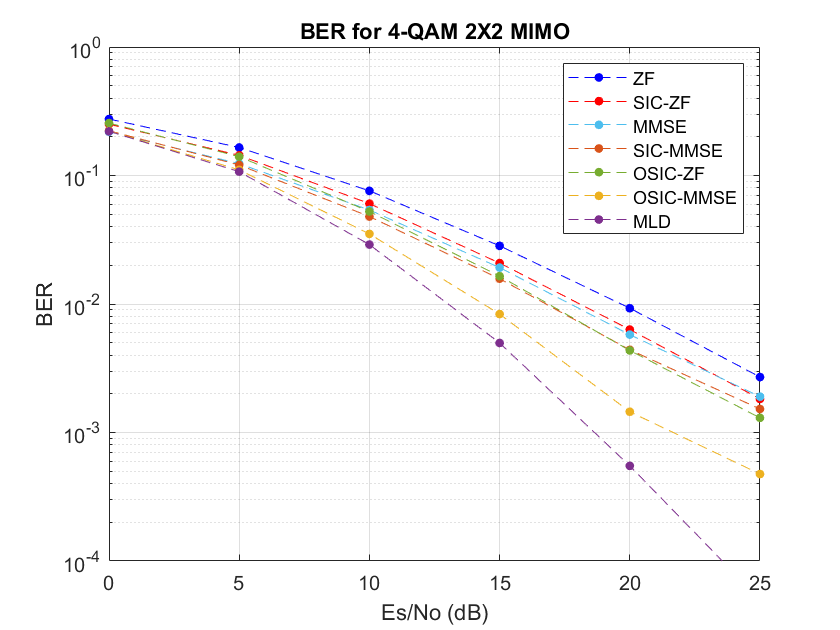
\includegraphics[width=1\textwidth]{BER_2x2_4qam.png}}
		\caption{BER}
	\end{subfigure}%
	\begin{subfigure}{0.5\textwidth}
		\centerline{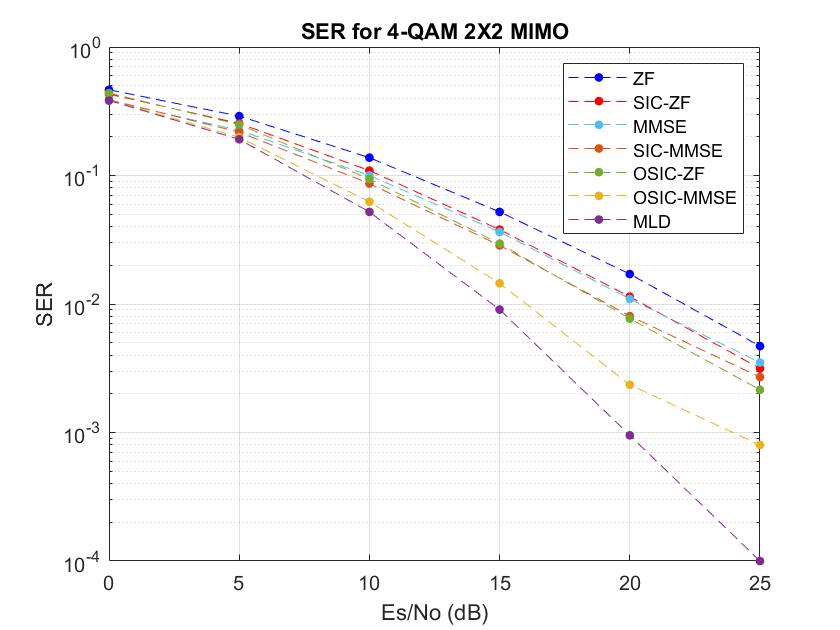
\includegraphics[width=1\textwidth]{SER_2x2_4qam.png}}
		\caption{SER}
	\end{subfigure}\\%
	\caption{4-QAM 2$\times$2 MIMO}
\end{figure}
\begin{figure}[H]
	\centering
	\begin{subfigure}{0.5\textwidth}
		\centerline{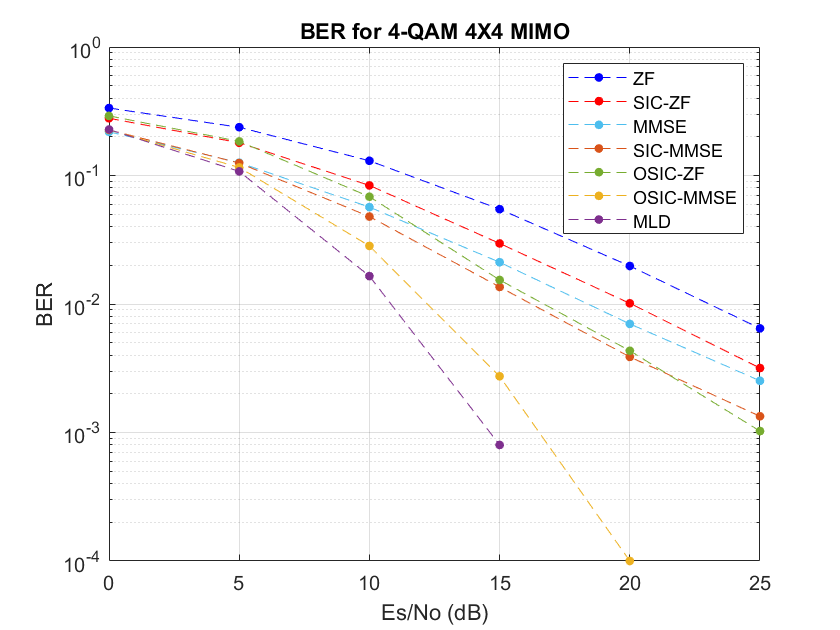
\includegraphics[width=1\textwidth]{BER_4x4_4qam.png}}
		\caption{BER}
	\end{subfigure}%
	\begin{subfigure}{0.5\textwidth}
		\centerline{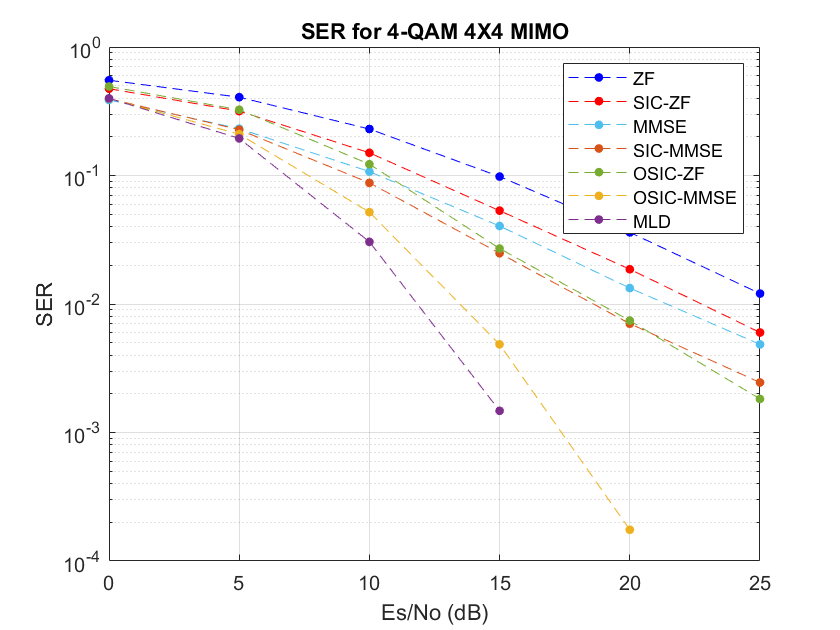
\includegraphics[width=1\textwidth]{SER_4x4_4qam.png}}
		\caption{SER}
	\end{subfigure}\\%
	\caption{4-QAM 4$\times$4 MIMO}
\end{figure}
\begin{figure}[H]
	\centering
	\begin{subfigure}{0.5\textwidth}
		\centerline{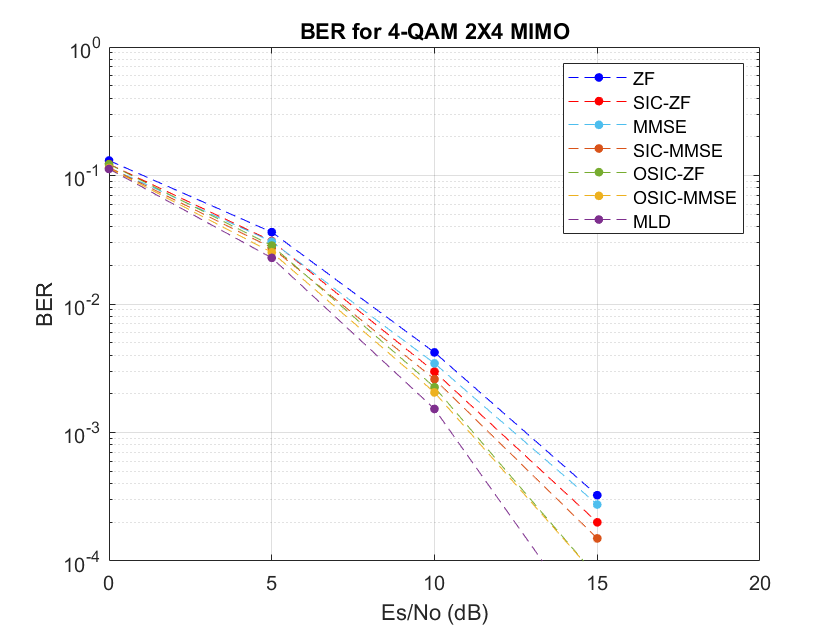
\includegraphics[width=1\textwidth]{BER_2x4_4qam.png}}
		\caption{BER}
	\end{subfigure}%
	\begin{subfigure}{0.5\textwidth}
		\centerline{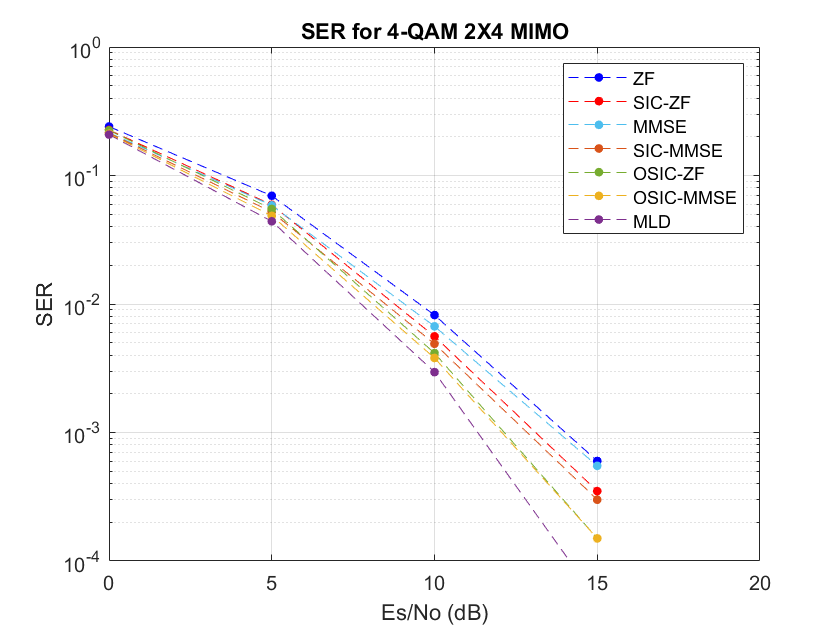
\includegraphics[width=1\textwidth]{SER_2x4_4qam.png}}
		\caption{SER}
	\end{subfigure}\\%
	\caption{4-QAM 2$\times$4 MIMO}
\end{figure}
% 16-QAM start
\begin{figure}[H]
	\centering
	\begin{subfigure}{0.5\textwidth}
		\centerline{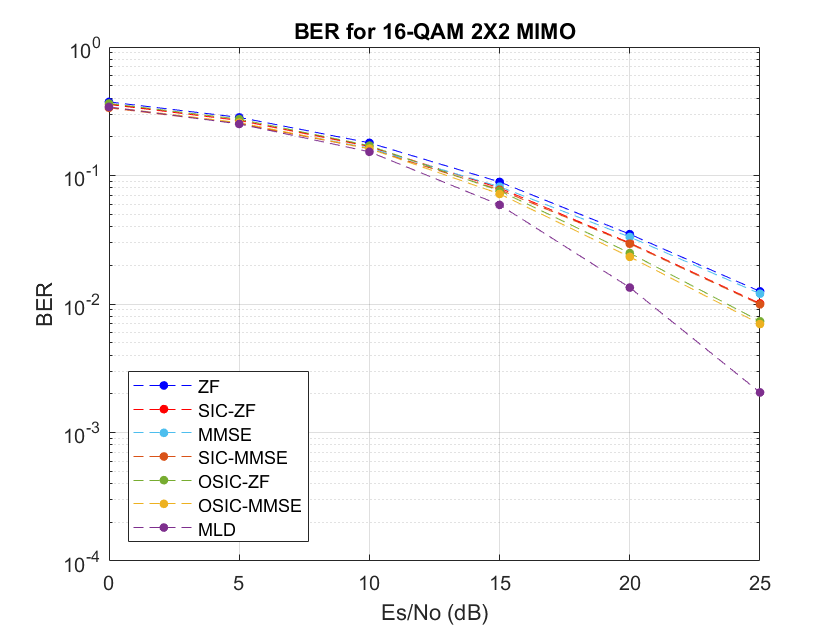
\includegraphics[width=1\textwidth]{BER_2x2_16qam.png}}
		\caption{BER}
	\end{subfigure}%
	\begin{subfigure}{0.5\textwidth}
		\centerline{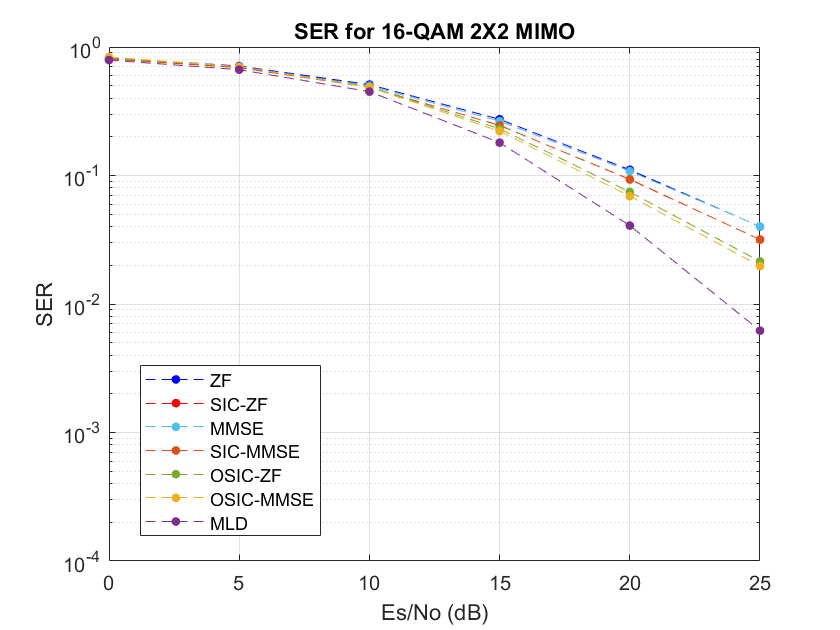
\includegraphics[width=1\textwidth]{SER_2x2_16qam.png}}
		\caption{SER}
	\end{subfigure}\\%
	\caption{16-QAM 2$\times$2 MIMO}
\end{figure}
\begin{figure}[H]
	\centering
	\begin{subfigure}{0.5\textwidth}
		\centerline{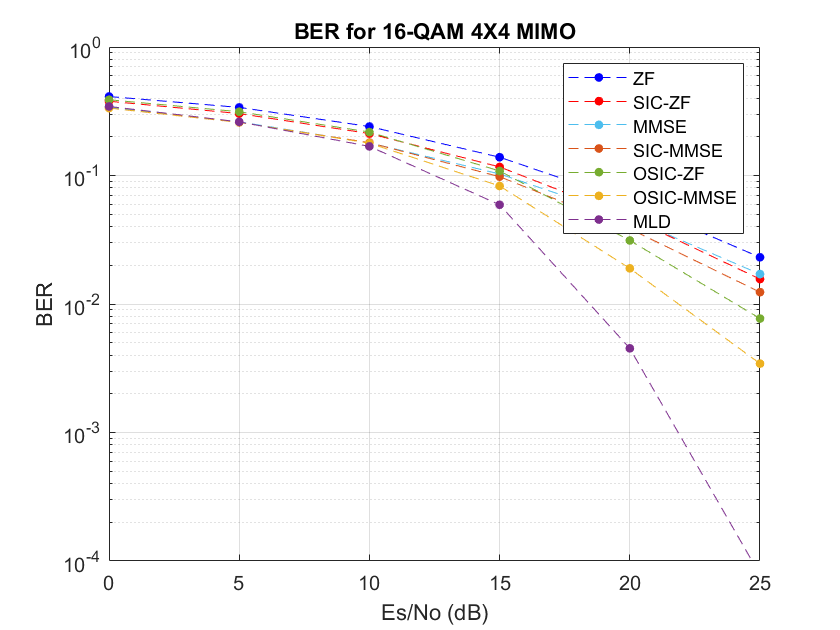
\includegraphics[width=1\textwidth]{BER_4x4_16qam.png}}
		\caption{BER}
	\end{subfigure}%
	\begin{subfigure}{0.5\textwidth}
		\centerline{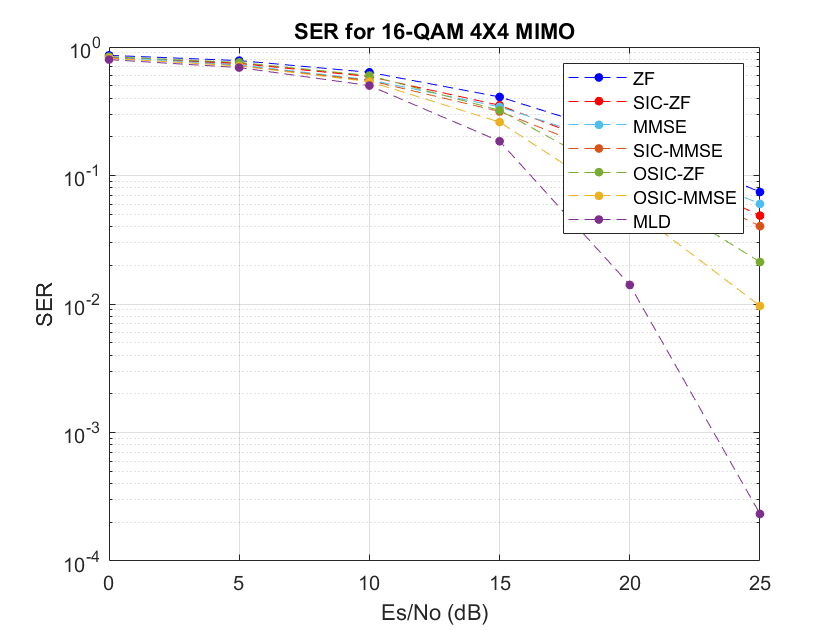
\includegraphics[width=1\textwidth]{SER_4x4_16qam.png}}
		\caption{SER}
	\end{subfigure}\\%
	\caption{16-QAM 4$\times$4 MIMO}
\end{figure}
\begin{figure}[H]
	\centering
	\begin{subfigure}{0.5\textwidth}
		\centerline{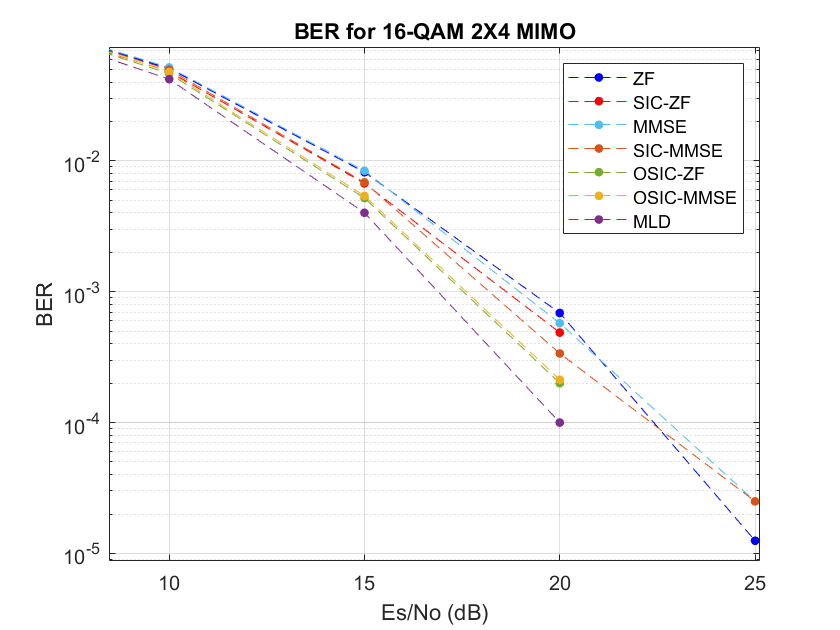
\includegraphics[width=1\textwidth]{BER_2x4_16qam.png}}
		\caption{BER}
	\end{subfigure}%
	\begin{subfigure}{0.5\textwidth}
		\centerline{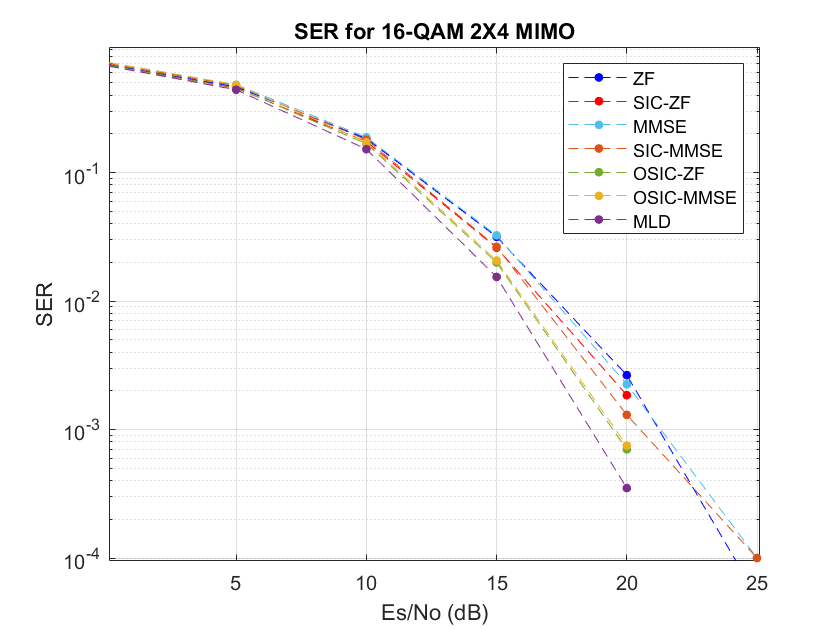
\includegraphics[width=1\textwidth]{SER_2x4_16qam.png}}
		\caption{SER}
	\end{subfigure}\\%
	\caption{16-QAM 2$\times$4 MIMO}
\end{figure}

\subsubsection{Eb/N0: 0$\sim$25dB}
\begin{figure}[H]
	\centering
	\begin{subfigure}{0.5\textwidth}
		\centerline{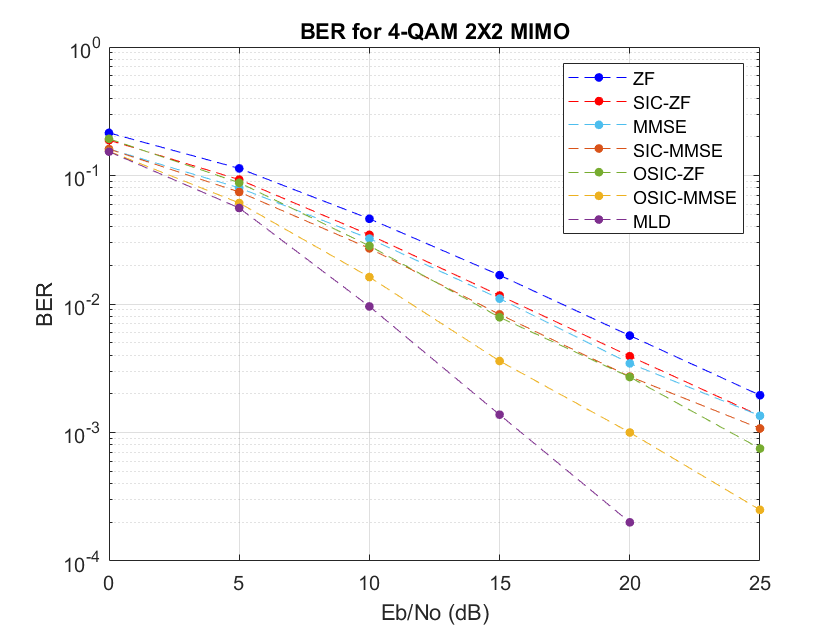
\includegraphics[width=1\textwidth]{BER_2x2_4qam2.png}}
		\caption{BER}
	\end{subfigure}%
	\begin{subfigure}{0.5\textwidth}
		\centerline{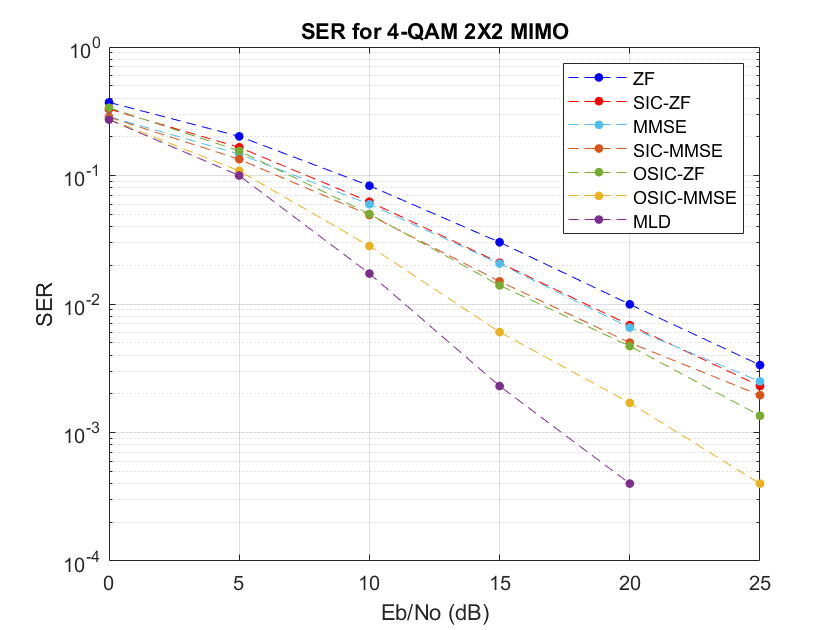
\includegraphics[width=1\textwidth]{SER_2x2_4qam2.png}}
		\caption{SER}
	\end{subfigure}\\%
	\caption{4-QAM 2$\times$2 MIMO}
\end{figure}
\begin{figure}[H]
	\centering
	\begin{subfigure}{0.5\textwidth}
		\centerline{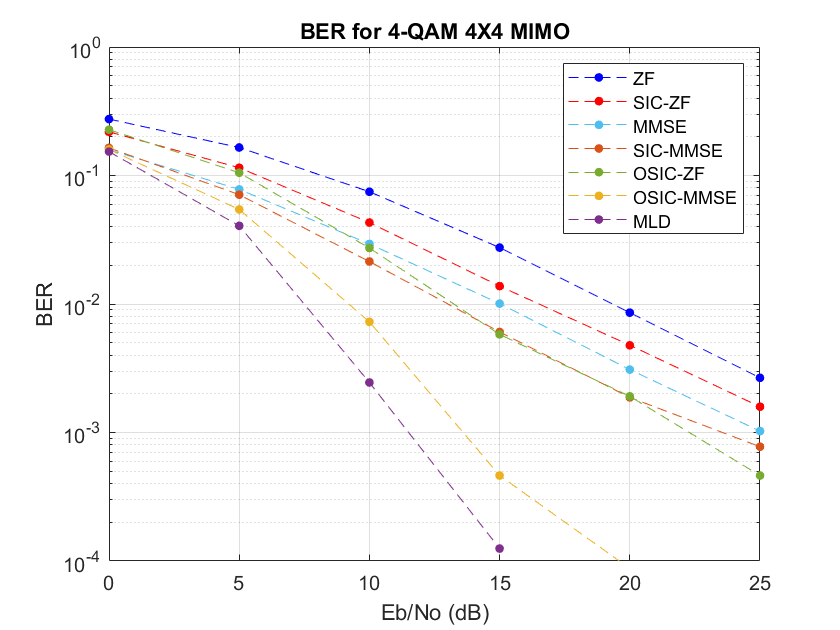
\includegraphics[width=1\textwidth]{BER_4x4_4qam2.png}}
		\caption{BER}
	\end{subfigure}%
	\begin{subfigure}{0.5\textwidth}
		\centerline{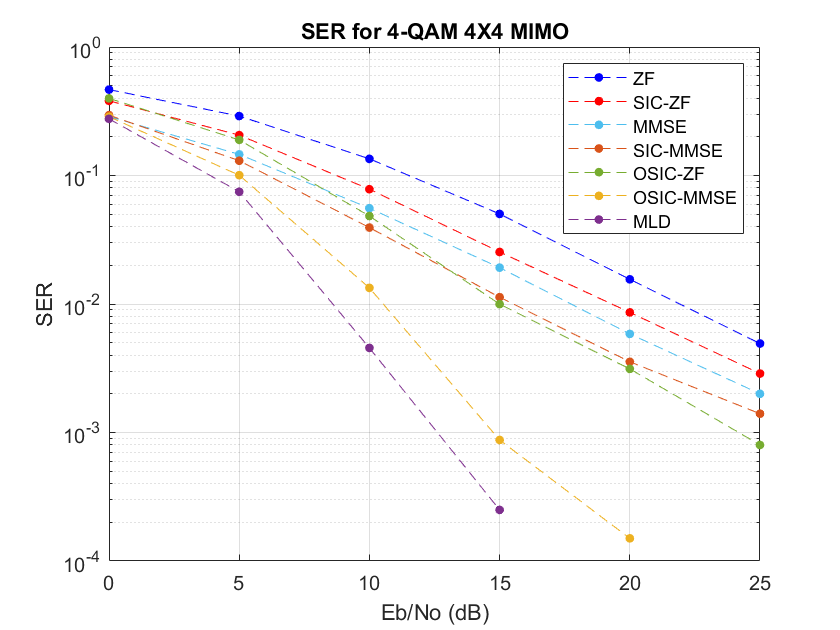
\includegraphics[width=1\textwidth]{SER_4x4_4qam2.png}}
		\caption{SER}
	\end{subfigure}\\%
	\caption{4-QAM 4$\times$4 MIMO}
\end{figure}
\begin{figure}[H]
	\centering
	\begin{subfigure}{0.5\textwidth}
		\centerline{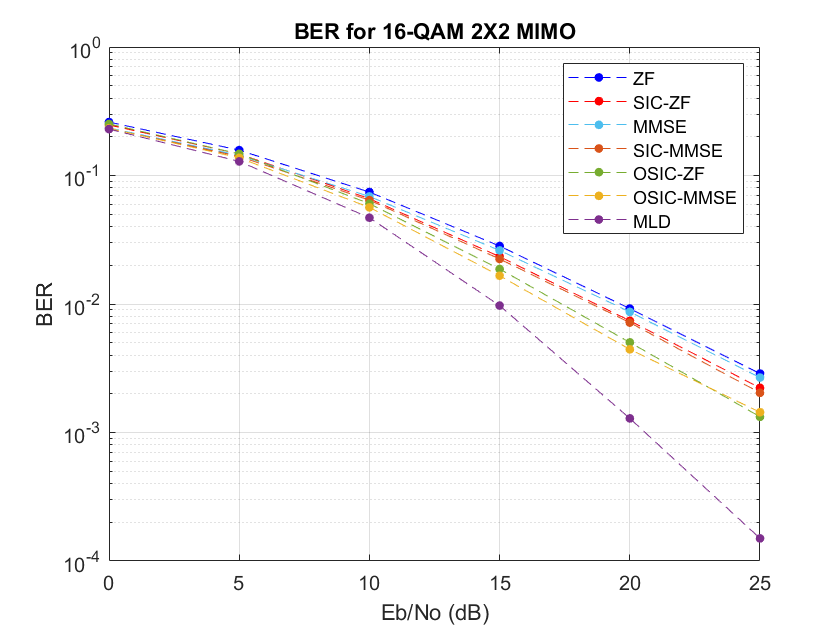
\includegraphics[width=1\textwidth]{BER_2x2_16qam2.png}}
		\caption{BER}
	\end{subfigure}%
	\begin{subfigure}{0.5\textwidth}
		\centerline{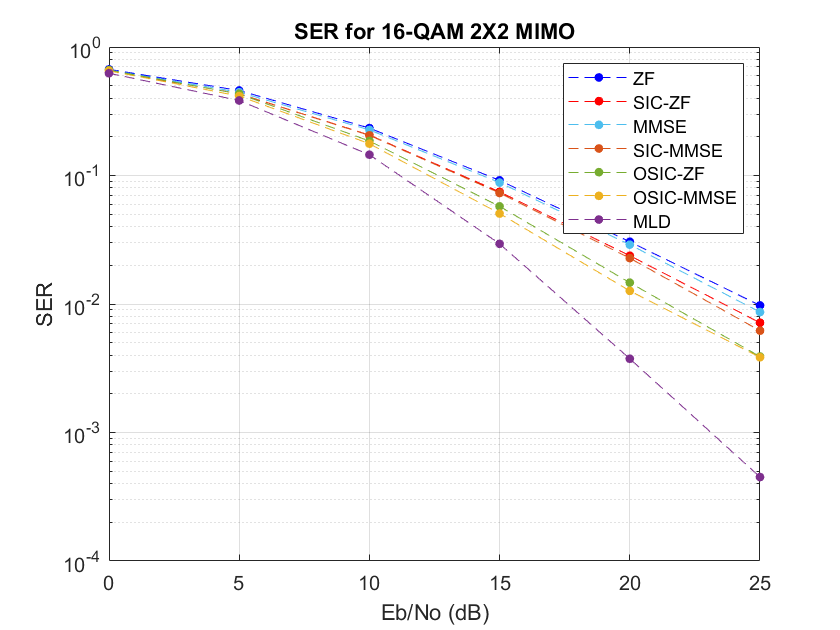
\includegraphics[width=1\textwidth]{SER_2x2_16qam2.png}}
		\caption{SER}
	\end{subfigure}\\%
	\caption{16-QAM 2$\times$2 MIMO}
\end{figure}
\begin{figure}[H]
	\centering
	\begin{subfigure}{0.5\textwidth}
		\centerline{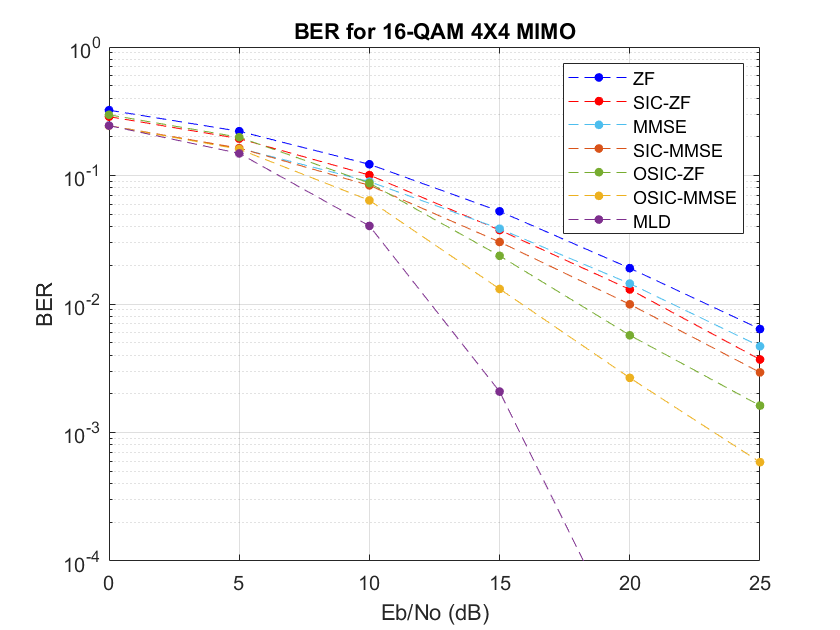
\includegraphics[width=1\textwidth]{BER_4x4_16qam2.png}}
		\caption{BER}
	\end{subfigure}%
	\begin{subfigure}{0.5\textwidth}
		\centerline{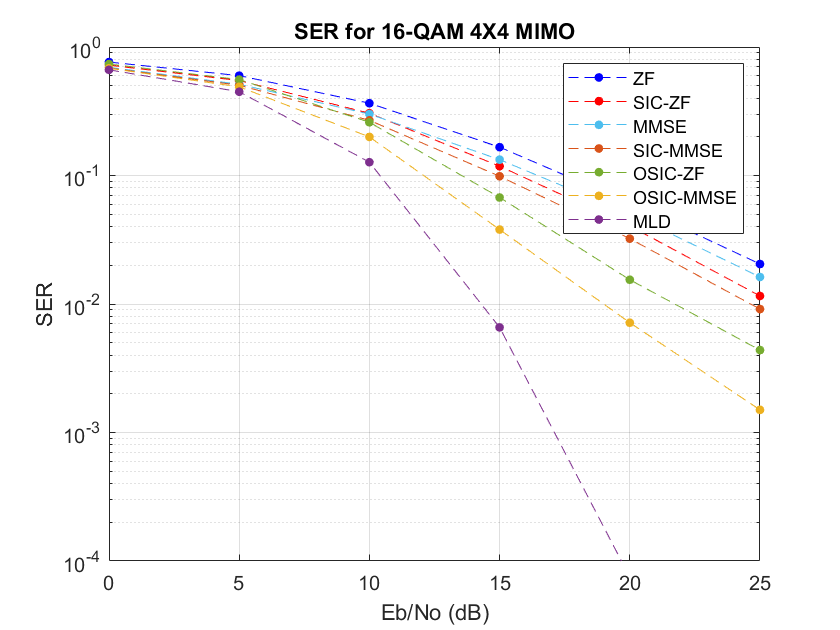
\includegraphics[width=1\textwidth]{SER_4x4_16qam2.png}}
		\caption{SER}
	\end{subfigure}\\%
	\caption{16-QAM 4$\times$4 MIMO}
\end{figure}
\subsubsection{Discussion}
$N_T$, 즉, transmit antenna의 개수가 많을수록  OSIC의 장점이 더욱 잘 들어난다. $N_T=2$일 때, 0.5의 확률로 SIC와 동일하게 작동하기 때문인 것으로 보인다.
\subsection{SIC의 Error Propagation}
다음은 \bd{SIC(MMSE)에서 $s_1$의 검출이 틀렸을 때 }$s_n$의 검출이 틀릴 확률을 실험적으로 얻은 결과이다.
\begin{table}[H]
\centering
\begin{tabular}{cccccc}
\toprule
\multicolumn{1}{c}{} & \multicolumn{1}{c}{\textbf{$2\times2$ MIMO}} & \multicolumn{1}{c}{\textbf{$2\times4$ MIMO}} & \multicolumn{3}{c}{\textbf{$4\times4$ MIMO}} \\
\cmidrule(rl){2-2} \cmidrule(rl){3-3} \cmidrule(rl){4-6}
\textbf{$E_s/N_0$(dB)} & {$n=2$} & {$n=2$} & {$n=2$} & {$n=3$} & {$n=4$}\\
\midrule
0 & 0.8055&0.7094& 0.8232 & 0.8176 & 0.7989\\
5 & 0.7182&0.5435&0.7291 & 0.7309 & 0.7234\\
10 & 0.6420&0.3972&0.6336 & 0.6347 & 0.6238\\
15 &0.5700&0.3314& 0.5545 & 0.5536 & 0.5586\\
20 & 0.5164&0.3422&0.5219 & 0.5213 & 0.5029\\
25 & 0.5000&0.1667&0.5303 & 0.5182 & 0.5043\\
\bottomrule
\end{tabular}
\caption{16-QAM $s_n$의 검출이 틀릴 확률}
\end{table}

\begin{table}[H]
\centering
\begin{tabular}{cccccc}
\toprule
\multicolumn{1}{c}{} & \multicolumn{1}{c}{\textbf{$2\times2$ MIMO}} & \multicolumn{1}{c}{\textbf{$2\times4$ MIMO}} & \multicolumn{3}{c}{\textbf{$4\times4$ MIMO}} \\
\cmidrule(rl){2-2} \cmidrule(rl){3-3} \cmidrule(rl){4-6}
\textbf{$E_s/N_0$(dB)} & {$n=2$} & {$n=2$} & {$n=2$} & {$n=3$} & {$n=4$}\\
\midrule
0 & 0.4705 & 0.3310 & 0.4189   & 0.4327  &  0.4568\\
5 & 0.4304 & 0.2801 & 0.3615  &  0.3624  &  0.3689\\
10 & 0.4084 & 0.2055 & 0.3571  &  0.3667   & 0.3484\\
15 & 0.4763 & 0.3333 &0.3984  &  0.3516  &  0.3438\\
20 & 0.4729 & NaN&0.3881 &   0.4030  &  0.3731\\
25 & 0.5385  & NaN&0.4222   & 0.5111 &   0.3556\\
\bottomrule
\end{tabular}
\caption{4-QAM $s_n$의 검출이 틀릴 확률}
\end{table}

\begin{table}[H]
\centering
\begin{tabular}{cccccc}
\toprule
\multicolumn{1}{c}{} & \multicolumn{1}{c}{\textbf{$2\times2$ MIMO}} & \multicolumn{3}{c}{\textbf{$4\times4$ MIMO}} \\
\cmidrule(rl){2-2} \cmidrule(rl){3-5}
\textbf{$E_s/N_0$(dB)} & {$n=2$} & {$n=2$} & {$n=3$} & {$n=4$}\\
\midrule
0 & 0.9460 & 0.9519  &  0.9480   & 0.9440\\
5 & 0.9027 &0.9206   & 0.9133 &   0.9055\\
10 & 0.8246 &  0.8611  &  0.8545  &  0.8413\\
15 & 0.7222 & 0.7568   & 0.7667  &  0.7526\\
20 & 0.6440 & 0.6628   & 0.6734 &   0.6682\\
25 & 0.5978  & 0.6038  &  0.6077  &  0.6148\\
\bottomrule
\end{tabular}
\caption{64-QAM $s_n$의 검출이 틀릴 확률}
\end{table}

\noindent
$N_R > N_T$일 때, \textsl{error propagation}의 영향이 확연히 줄어든 것을 확인할 수 있었다.

\subsection{SNR에 따른 SER/BER 변화 추이}
다음은 $10^5$번의 iteration을 반복한 결과이다. (하나의 iteration에서는 모든 송신 안테나가 동시에 각각 단 하나의 신호 송신 \& frequency flat fading)
\begin{figure}[H]
	\centering
	\begin{subfigure}{0.5\textwidth}
		\centerline{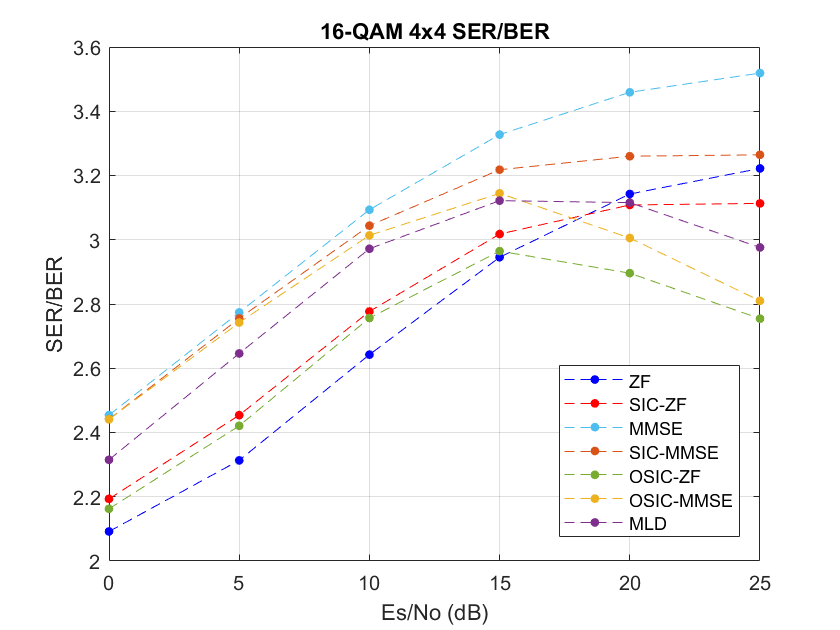
\includegraphics[width=1\textwidth]{ser_div_ber.png}}
		\caption{BER}
	\end{subfigure}%
	\begin{subfigure}{0.5\textwidth}
		\centerline{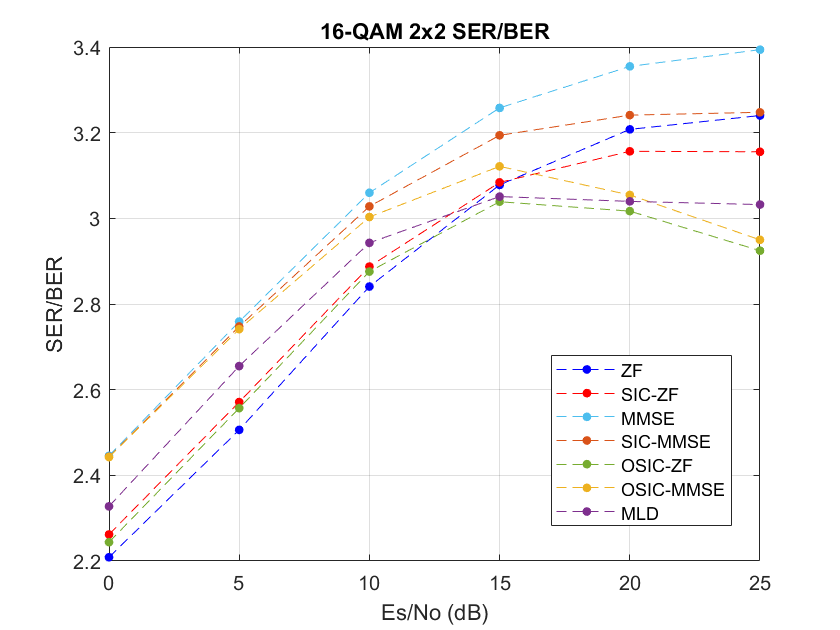
\includegraphics[width=1\textwidth]{ser_div_ber_2.png}}
		\caption{SER}
	\end{subfigure}\\%
	\caption{16-QAM 4$\times$4 MIMO}
\end{figure}
\noindent
\bd{Discussion}

높은 SER/BER은 signal error당 bit error는 적다는 것이다. Signal error가 있다고 하더라도 해당 signal에서 발생하는 bit error는 적다는 의미로 분석된다. 반대로, SER/BER이 낮다는 것은 signal error당 bit error가 높다는 의미로 분석된다.

SNR이 높아질수록 noise의 간섭(interference)가 작어지기 때문에 SER/BER이 높아지는 것은 예상할 수 있는 결과이다.\\
\\
\bd{OSIC와 MLD에서 SER/BER이 증가하다가 떨어지는} 원인에 대해서는 추가적인 분석이 필요할 것 같다.

\section{미해결 \& 추가연구 필요 내용}
\begin{itemize}
	\item \bd{Table 2}를 보면 SNR이 증가했음에도 불구하고 $s_n$의 검출에 오류가 있을 확률이 증가하기도 하는 모습을 볼 수 있다. 이것이 단순히 낮은 iteration에 의한 결과인지, 다른 이유에 의한 결과인지 추가적으로 연구해볼 필요가 있을 것 같다.
	\item 어떤 receiver를 사용하는지와 상관없이 SER/BER은 지속적으로 오르다가 $\log_{2}M$에 수렴할 것으로 예상했다. OSIC의 경우 SER/BER 값이 오르다가 다시 떨어지는 모습을 보였다. 그 원인에 대해 파악하지 못했다.
\end{itemize}

\section[Entire Code]{Entire Code \footnote{Uploaded on https://github.com/lightwick/ICS$\textunderscore $project/tree/main/Successive$\textunderscore $Cancellation}}
\bd{ZF, MMSE, MLD에 대한 코드 생략...}\\
\newgeometry{margin=1cm, bottom=0.5cm}
\noindent\bd{main.m}
\begin{lstlisting}[style=Matlab-editor, frame=single, numbers=left,]
close all
clear all
clc
dbstop if error
dbstop if warning

addpath('../tools/')

% Environment Varible
M = 16
Nt = 4
Nr = 4
NumberIteration = 10^4;

% Simulation
LengthBitSequence = Nt * log2(M); % log2(M) bits per signal
LengthSignalSequence = Nt;

% EbN0_dB = 0:5:25;
% EbN0 = db2pow(EbN0_dB);
% 
% EsN0 = EbN0 * log2(M);
% EsN0_dB = pow2db(EsN0);

EsN0_dB = 0:5:25;
EsN0 = db2pow(EsN0_dB);

EbN0 = EsN0 / log2(M);
EbN0_dB = pow2db(EbN0);

% BitErrorCount_ZF = zeros(1, length(EsN0_dB));
% SignalErrorCount_ZF = zeros(1, length(EsN0_dB));
% BitErrorCount_MLD = zeros(1, length(EsN0_dB));
% SignalErrorCount_MLD = zeros(1, length(EsN0_dB));
% 
% BitErrorCount_MMSE = zeros(1, length(EsN0_dB));
% SignalErrorCount_MMSE = zeros(1, length(EsN0_dB));

BitErrorCount = zeros(7, length(EsN0_dB));
SignalErrorCount = zeros(7, length(EsN0_dB));

NormalizationFactor = sqrt(2/3*(M-1)*Nt);

BEC_tmp = zeros(size(BitErrorCount));
SEC_tmp = zeros(size(SignalErrorCount));
    
FivePercent = ceil(NumberIteration/20);
    
for iTotal = 1 : NumberIteration
    if mod(iTotal-100, FivePercent)==0
        tic
    end
    % Bit Generation
    SignalSequence = randi([0 M-1], Nt, 1);
    SignalBinary = de2bi(SignalSequence, log2(M), 'left-msb');
    SymbolSequence = qammod(SignalSequence, M) / NormalizationFactor;
    
    NoiseSequence = (randn(Nr, 1) + 1j * randn(Nr, 1)) / sqrt(2); % Noise (n) Generation
    H = (randn(Nr, Nt) + 1j * randn(Nr, Nt)) ./ sqrt(2); % Receiver x Transmitter

    for indx_EbN0 = 1 : length(EsN0)
        BEC = zeros(size(BitErrorCount,1), 1);
        SEC = zeros(size(SignalErrorCount,1), 1);
        % Received Signal (y = hs + n) Generation
        ReceivedSymbolSequence = H * SymbolSequence + NoiseSequence * sqrt(1 / EsN0(indx_EbN0)); % log2(M)x1 matrix
        
        [Error, General_Error] = error_propagation_2(ReceivedSymbolSequence, SignalSequence, SignalBinary,  M, H, EsN0, ReceiverType)
        
        % ZF
        [BEC(1), SEC(1)] = simulate_zf(ReceivedSymbolSequence, SignalSequence, SignalBinary, M, H);
        
        % ZF - SIC
        [BEC(2), SEC(2)] = simulate_sic(ReceivedSymbolSequence, SignalSequence, SignalBinary,  M, H, EsN0(indx_EbN0), 'zf');
        
        % MMSE
        [BEC(3), SEC(3)] = simulate_mmse(ReceivedSymbolSequence, SignalSequence, SignalBinary, M, H, EsN0(indx_EbN0));
                
        % MMSE - SIC
        [BEC(4), SEC(4)] = simulate_sic(ReceivedSymbolSequence, SignalSequence, SignalBinary,  M, H, EsN0(indx_EbN0), 'mmse');
        
        % ZF - OSIC
        [BEC(5), SEC(5)] = simulate_osic(ReceivedSymbolSequence, SignalSequence, SignalBinary,  M, H, EsN0(indx_EbN0), 'zf');

        % MMSE - OSIC
        [BEC(6), SEC(6)] = simulate_osic(ReceivedSymbolSequence, SignalSequence, SignalBinary,  M, H, EsN0(indx_EbN0), 'mmse');
                
        % MLD Receiver
        [BEC(7), SEC(7)] = simulate_mld(ReceivedSymbolSequence, SignalSequence, SignalBinary,  M, H);
        
        BEC_tmp(:, indx_EbN0) = BEC;
        SEC_tmp(:, indx_EbN0) = SEC;
    end
    BitErrorCount = BitErrorCount + BEC_tmp;
    SignalErrorCount = SignalErrorCount + SEC_tmp;
    
    if mod(iTotal-100, FivePercent)==0
        ElapsedTime = toc;
        EstimatedTime = (NumberIteration-iTotal)*ElapsedTime;
        disp(sprintf("%d%%, estimated wait time %d minutes %d seconds", round(iTotal/NumberIteration*100), floor(EstimatedTime/60), floor(mod(EstimatedTime, 60))))
    end
end

BER = BitErrorCount / (LengthBitSequence * NumberIteration);
SER = SignalErrorCount / (LengthSignalSequence * NumberIteration);

% Plot
BER_Title = sprintf("BER for %d-QAM %dX%d MIMO", M, Nt, Nr);
SER_Title = sprintf("SER for %d-QAM %dX%d MIMO", M, Nt, Nr);
x_axis = "Es/No (dB)";

legend_order = ["ZF", "SIC-ZF", "MMSE", "SIC-MMSE", "OSIC-ZF", "OSIC-MMSE", "MLD"];
myplot(EsN0_dB, BER, BER_Title, x_axis, "BER", legend_order);
ylim([10^(-4) 1])
myplot(EsN0_dB, SER, SER_Title, x_axis, "SER", legend_order);
ylim([10^(-4) 1])
\end{lstlisting}
\noindent\bd{simulate\textunderscore sic.m}
\begin{lstlisting}[style=Matlab-editor, frame=single, numbers=left,]
function [BitErrorCount, SignalErrorCount] = simulate_sic(ReceivedSymbolSequence, SignalSequence, SignalBinary,  M, H, EsN0, ReceiverType)
    Nt = size(H,2);
    Nr = size(H,1);
    NormalizationFactor = sqrt(2/3*(M-1) * Nt); % size(H,1) = Nt
    persistent alphabet;
    if isempty(alphabet)
        alphabet = qammod([0:M-1], M) / NormalizationFactor;
    end
    DetectedSignalSequence = zeros(Nt,1);
    for ii = 1:Nt
        if strcmp(ReceiverType, 'zf')
            w = NormalizationFactor * pinv(H); % pinv(H) = inv(H' * H) * H'
        else
            w = NormalizationFactor * inv(H' * H + size(H,2) / EsN0 * eye(size(H,2))) * H';
        end
        w = w(1,:);
        DetectedSymbol = w * ReceivedSymbolSequence;
        DetectedSignal = qamdemod(DetectedSymbol, M);
        DetectedSignalSequence(ii, 1) = DetectedSignal;
        
        %% Remove the effect of the regarded transmit antenna
        RemodulatedSignal = alphabet(DetectedSignal+1);
        ReceivedSymbolSequence = ReceivedSymbolSequence - H(:,1) * RemodulatedSignal;
        H(:,1) = []; % remove first column
    end
    DetectedBinary = de2bi(DetectedSignalSequence, log2(M), 'left-msb');
    BitErrorCount = sum(SignalBinary~=DetectedBinary, 'all');
    SignalErrorCount = sum(SignalSequence~=DetectedSignalSequence, 'all');
end

\end{lstlisting}
\noindent\bd{simulate\textunderscore osic.m}
\begin{lstlisting}[style=Matlab-editor, frame=single, numbers=left,]
function [BitErrorCount, SignalErrorCount] = simulate_osic(ReceivedSymbolSequence, SignalSequence, SignalBinary,  M, H, EsN0, ReceiverType)
    Nt = size(H,2);
    Nr = size(H,1);
    NormalizationFactor = sqrt(2/3*(M-1) * Nt);
    persistent alphabet
    if isempty(alphabet)
        alphabet = qammod([0:M-1], M) / NormalizationFactor;
    end
    snr = EsN0 / (NormalizationFactor^2);
    DetectedSignalSequence = zeros(Nt,1);
    
    HasValue = false(Nt,1);
    
    for ii = 1:Nt
        if strcmp(ReceiverType, 'zf')
            w = NormalizationFactor * pinv(H); % pinv(H) = inv(H' * H) * H'
        else
            w = NormalizationFactor * inv(H' * H + size(H,2) / EsN0 * eye(size(H,2))) * H';
        end
        wH_squared = abs(w*H).^2;
        
        %% Get Biggest SINR
        sinr = snr*diag(wH_squared)./(snr*(sum(wH_squared,2) - diag(wH_squared))+sum(abs(w).^2,2));
        [~,idx] = max(sinr);
        DetectedSymbol = w(idx, :) * ReceivedSymbolSequence;
        DetectedSignal = qamdemod(DetectedSymbol, M);
        
        OriginalIndex = get_original_index(HasValue, idx);
        DetectedSignalSequence(OriginalIndex, 1) = DetectedSignal;
        HasValue(OriginalIndex) = true;
        
        %% Remove the effect of the regarded transmit antenna
        RemodulatedSignal = alphabet(DetectedSignal+1);
        ReceivedSymbolSequence = ReceivedSymbolSequence - H(:,idx) * RemodulatedSignal;
        H(:,idx) = []; % remove column
    end
    DetectedBinary = de2bi(DetectedSignalSequence, log2(M), 'left-msb');
    BitErrorCount = sum(SignalBinary~=DetectedBinary, 'all');
    SignalErrorCount = sum(SignalSequence~=DetectedSignalSequence, 'all');
end

function OriginalIndex = get_original_index(HasValue, idx)
    OriginalIndex = 0;
    while idx
        OriginalIndex = OriginalIndex + 1;
        if ~HasValue(OriginalIndex)
            idx = idx - 1;
        end
    end
end
\end{lstlisting}
\noindent\bd{myplot.m}
\begin{lstlisting}[style=Matlab-editor, frame=single, numbers=left,]
function fig = myplot(x, y, title_in, xlabel_in, ylabel_in, legend_in)
    colors = ["#0000FF", "#FF0000", "#4DBEEE", "#D95319", "#77AC30", "#EDB120", "#7E2F8E"];
    
    fig = figure();
    semilogy(x, y(1,:), '.--', 'Color', colors(1),'MarkerSize', 15);
    hold on
    for ii=2:size(y,1)
        semilogy(x, y(ii,:), '.--','Color', colors(ii), 'MarkerSize', 15);
    end
    ylabel(ylabel_in);
    title(title_in);
    grid on
    legend(legend_in);
    xlabel(xlabel_in);
end    
\end{lstlisting}
\end{document}